\subsection{Pitfalls and more granular analysis on the Russell 2000}

Unfortunately those results are not very conclusive, the static Hurst exponent is not a very robust statistic and can be
influenced by the length of the series, the presence of trends, or the presence of structural breaks.
To highlight these shortcomings, we adjust both the analysis frequency and the study period. Specifically, we perform a
detailed investigation across different frequencies (daily, weekly, monthly) and various study periods, comparing the
outcomes. This combined approach enables us to detect long-memory behavior within particular timeframes and ensures
more robust and reliable conclusions.

\begin{table}[h!]
    \centering
    \pgfplotstabletypeset[
        col sep=comma,
        header=true,
        string type,
        every head row/.style={before row=\hline, after row=\hline},
        every last row/.style={after row=\hline},
        columns/Frequency/.style={column name=Frequency, string type},
        columns/Hurst exponent/.style={column name=Hurst exponent, fixed, precision=2},
        columns/modified Hurst exponent/.style={column name=modified Hurst exponent, fixed, precision=3},
        columns/critical value/.style={column name=critical value, fixed, precision=3},
        columns/long memory/.style={column name=long memory, fixed, precision=3},
    ] {data/frequencies_results.csv}
    \caption{Results for Hurst exponent, modified Hurst exponent, critical value at 10\% and rejection of the null
    hypothesis of long memory, different frequencies daily, weekly and montlhy from 1987-09-10 to 2025-02-28.}
    \label{tab:frequencies_results}
\end{table}

\FloatBarrier

\begin{table}[h!]
    \centering
    \pgfplotstabletypeset[
        col sep=comma,
        header=true,
        string type,
        every head row/.style={before row=\hline, after row=\hline},
        every last row/.style={after row=\hline},
        columns/Period/.style={column name=Period, string type},
        columns/Hurst exponent/.style={column name=Hurst exponent, fixed, precision=2},
        columns/modified Hurst exponent/.style={column name=modified Hurst exponent, fixed, precision=3},
        columns/critical value/.style={column name=critical value, fixed, precision=3},
        columns/long memory/.style={column name=long memory, fixed, precision=3},
    ] {data/timestamp_analysis.csv}
    \caption{Results for Hurst exponent, modified Hurst exponent, critical value at 10\% and rejection of the null
    hypothesis of long memory, different estimation periods on monthly data from 1987-09-10 to 2025-02-28}
    \label{tab:timestamp_analysis}
\end{table}

\FloatBarrier

The results indicate that the detection of long memory strongly depends on the frequency and period of analysis.
At daily and weekly frequencies, the Hurst exponents are close to 0.5, suggesting no long memory, while at the monthly
frequency, a persistent behavior is detected (H = 0.645). Regarding estimation periods, only the longest period
(1987-2025) indicates long memory, whereas more recent periods reject this hypothesis. This suggests that long memory
may be an unstable characteristic influenced by structural trends or market changes.


The long memory properties of the Russell 2000 index are not stable over time and may be influenced by
structural changes or market dynamics. Given that the presence of long memory is not a consistent feature of the series,
it is necessary to delve into a more nuanced analysis.

We can distinguish two main contributions to the multifractal spectrum:
\[
\mathcal{M}(q) \propto \underbrace{f_{\text{corr}}(q)}_{\substack{\text{Temporal correlations} \\ \text{in the series}}} + \underbrace{f_{\text{tail}}(q)}_{\substack{\text{Strongly non-Gaussian} \\ \text{distribution}}}
\]

Therefore, in the literature, the multifractality is often reffered as two types :

Type I multifractality stems from long-range correlations within the time series, whereas Type II multifractality arises
from a broad probability density function of the series values Jan W. Kantelhardt (2002) and al. This distinction enables us to identify and quantify
the type of multifractality present. By shuffling the series, we effectively eliminate the long-range correlations,
retaining only the influence of the value distribution. In an ideal monofractal series, the Hölder exponent would peak
at 0.5 thus, the difference between the exponents of the original and shuffled series reflects the contribution of
long-range correlations to the multifractality. Moreover, if the shuffled series still exhibits a Hölder exponent
greater than 0.5, this suggests the presence of Type II multifractality.



\subsection{Rolling critical value}

To further investigate the long memory properties of the Russell 2000 index,
we perform a ten year rolling analysis of the modified R/S statistic and compare it to the critical value at the
10\% significance level (1.620).


\begin{figure}[htbp]
    \centering
    \begin{tikzpicture}
        %--- Premier axe (pour le tracé uniquement) ---
        \begin{axis}[
            name=axis1,
            width=\textwidth,
            height=8cm,
            date coordinates in=x,
            xticklabel=\year-\month,
            xticklabel style={rotate=45, anchor=east},
            grid=major,
            xlabel={Date},
            ylabel={Price},
            ymin=3, ymax=8, % Échelle de gauche
            % (aucune légende ici)
        ]
            \addplot[
                blue!50,
                thick
            ] table[
                x=Date,
                y={Price},
                col sep=comma
            ] {data/rolling_and_price.csv};
        \end{axis}

        %--- Deuxième axe (inclut la légende globale) ---
        \begin{axis}[
            name=axis2,
            at={(axis1.south west)},
            anchor=south west,
            width=\textwidth,
            height=8cm,
            date coordinates in=x,
            xticklabel=\empty,  % On ne réaffiche pas les dates
            axis x line=none,   % Pas d'axe x sur le 2e graphique
            axis y line=right,  % Axe y à droite
            ymin=0.6, ymax=3, % Échelle de droite
            ylabel={Rolling modified R/S statistic},
            yticklabel style={color=purple},  % Couleur rappelée pour la courbe
            ylabel style={color=purple},
            grid=major,
            legend to name=global, % On prépare la légende globale
            legend style={
                font=\footnotesize,
                legend columns=3
            },
        ]
            % Réintégrer l'entrée de légende pour la courbe bleue
            \addlegendimage{blue!50, thick}
            \addlegendentry{Russell  2000 prices}

            %--- Alpha Width ---
            \addplot[
                green,
                thick
            ] table[
                x=Date,
                y={Critical Value},
                col sep=comma
            ] {data/rolling_and_price.csv};
            \addlegendentry{Rolling modified R/S statistic}

            %--- Threshold ---
            \addplot[
                red,
                thick,
                dashed
            ] coordinates {
                ({1997-09-30}, 1.620)
                ({2025-02-28}, 1.620)
            };
            \addlegendentry{Threshold (V=1.620)}
        \end{axis}

        % Placement de la légende globale sous les axes
        \node at (current bounding box.south) [below=1cm]
            {\pgfplotslegendfromname{global}};
    \end{tikzpicture}
    \caption{Rolling modified R/S statistic (green) et alpha width (purple).
Both metrics are computed using a ten-year rolling window on monthly data.}
\end{figure}

\FloatBarrier

Therefore, only one period in 2009 exhibits long memory, while the rest of the series remains below the critical value.

\section{Markov Switching Multifractal (MSM)}
\label{sec:msm}

In the Markov Switching Multifractal (MSM) model introduced by Calvet and Fisher (2004), the volatility process is driven by a product of $K$ independent components (or multipliers), each evolving according to a Markov chain. Specifically, for each level $k = 1, \ldots, K$, the multiplier $M_{k,t}$ can take one of two values, for instance $m_0$ or $(2 - m_0)$, ensuring the mean of the two states equals 1. This binomial structure leads to a total of $2^K$ possible configurations (states) at time $t$.

\subsection{Model Specification}
Let $\{ x_t \}$ be the log-returns of the asset. The MSM model posits:
\begin{equation}
    x_t \;=\; \sigma \,\sqrt{\prod_{k=1}^K M_{k,t}} \;\epsilon_t,\quad
    \epsilon_t \,\sim\, \mathcal{N}(0,1),
\end{equation}
where $\sigma$ is a global scale parameter and $M_{k,t}$ denotes the multiplier at level $k$. Each multiplier switches between its two possible values with probability $\gamma_k$, which often follows the decreasing scheme:
\begin{equation}
    \label{eq:gamma_k}
    \gamma_k \;=\; 1 \;-\; \bigl(1 - \gamma_1\bigr)^{b^{\,k-1}},
\end{equation}
for some $0 < \gamma_1 < 1$ and $b \in  [1,+\infty]$. Consequently, higher levels $k$ switch more frequently, introducing persistent high-frequency shocks to volatility.


\subsection{Probability of Switching}

\begin{figure}[!ht]
    \centering
    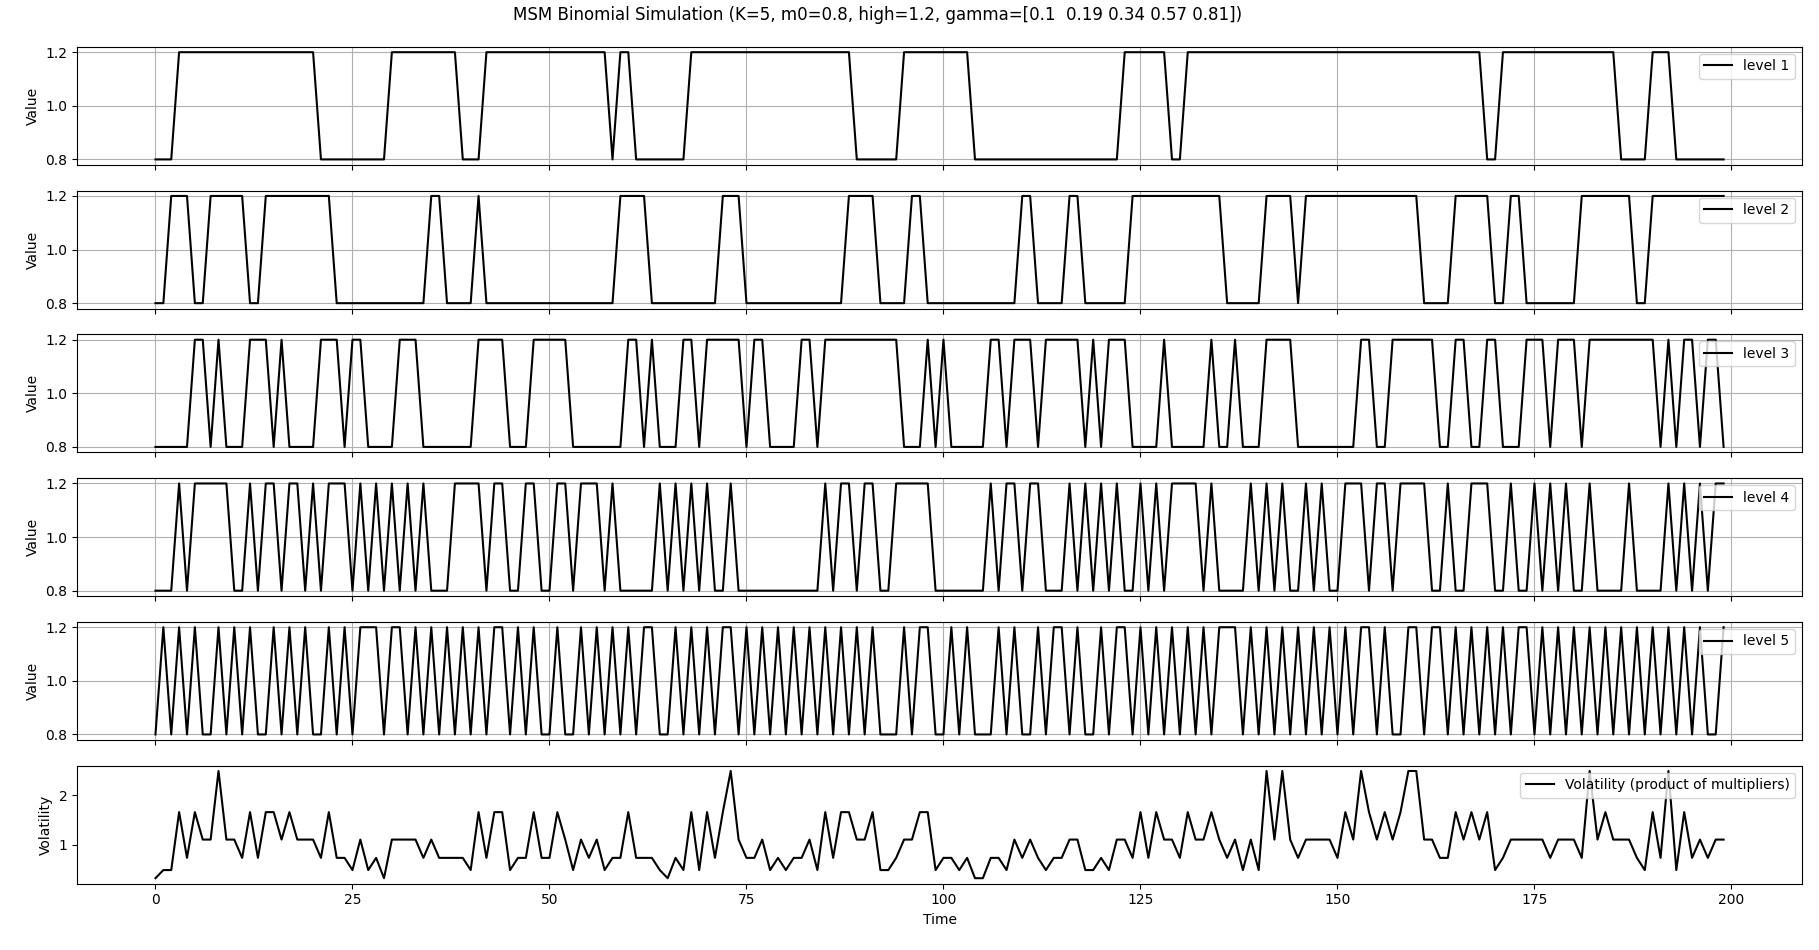
\includegraphics[width=0.8\textwidth]{img/k_analysis}
    \caption{Probability of switching at each k level in the MSM model, from top to bottom show increasing values of k.
    The simulation was performed for K=5, m0 = 0.8, 2-m0 = 1.2 and gamma [0.1, 0.19 0.34 0.57 0.81].}
    \label{fig:k_analysis}
\end{figure}

\FloatBarrier

Low-frequency multipliers $m_{t,k}$ build a fundamental block for persistent volatility.
A change in these low-level multipliers implies a strong tendency for movements in multiplied volatility.

Intermediate-frequency multipliers $m_{t,k}$ provide a smoother transition of volatility states,
effectively playing the role of a moving average in volatility. The resulting volatility may exhibit
clustering, largely due to highly correlated volatility components across different time scales.


High-frequency multipliers $m_{t,k}$ introduce additional outliers by directly affecting the
tails of the MSMF process (CalvetFisher2005). These volatility components are very short-lived and,
in extreme cases, resemble noise. As a result, it is not straightforward to capture the effect of this
component above certain thresholds of $\bar{k}$.

\subsection{Transition Dynamics and Likelihood}
Since each $M_{k,t}$ follows a two-state Markov chain, the joint process $\bigl(M_{1,t}, \dots, M_{K,t}\bigr)$ has $2^K$ states. We construct a $2^K \times 2^K$ transition matrix $\mathbf{A}$ encoding the probabilities of switching or staying in the same value at each level. The stationary distribution of $\mathbf{A}$ provides the initial state probabilities for the filtering procedure.

To estimate model parameters $(m_0,\,\gamma_1,\,b,\,\sigma)$, we maximize the log-likelihood of the observed returns. Let $\pi_t$ be the probability distribution over the $2^K$ states at time $t$. The likelihood is updated recursively via a forward filter:
\begin{enumerate}
    \item Compute the conditional density of $x_t$ given each state $s_j$,
          using $\sigma \sqrt{\prod_{k=1}^K M_{k,t}^{(j)}}$ as the volatility.
    \item Propagate $\pi_{t-1}$ through $\mathbf{A}$ and weight by the conditional densities.
    \item Normalize to obtain $\pi_t$ and accumulate the log-likelihood.
\end{enumerate}
This procedure iterates over all observations $x_1,\ldots,x_T$, yielding the maximum-likelihood estimates for the MSM parameters once the log-likelihood is maximized.

The MSM framework captures volatility clustering through a cascade of multiplicative factors, each operating on different timescales. Fast-switching levels introduce short-term fluctuations, while slow-switching levels generate persistent volatility regimes. As shown by Calvet and Fisher (2004), this hierarchical structure can replicate a wide range of stylized facts observed in financial returns, such as fat-tailed distributions and long-memory effects in volatility.





\subsection{MSM for depicting volatility}

\begin{figure}[!ht]
    \centering
    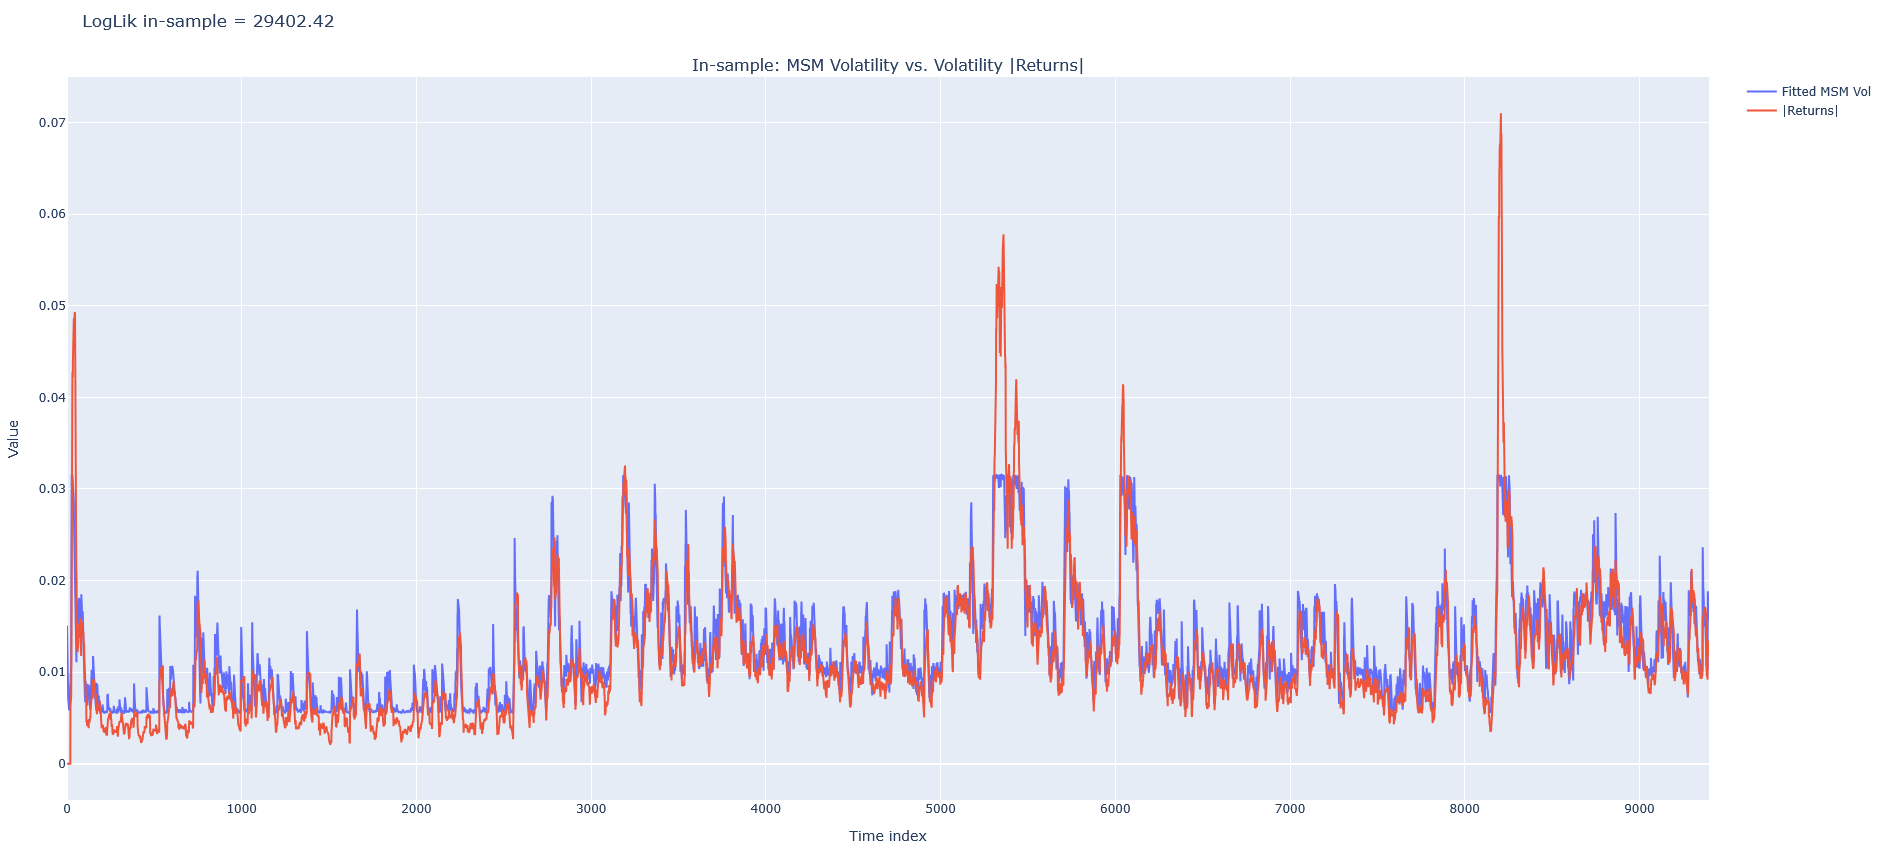
\includegraphics[width=0.8\textwidth]{img/msm_vol}
    \caption{Fitted volatility in sample and volatility of Russell  2000 returns, with MSM.}
    \label{fig:msm_fitted_vol}
\end{figure}

\FloatBarrier

Best param (m0, gamma1, sigma) = (0.46842105263157896, 0.01, 0.01663157894736842) \\

LogLik = 29402.418073294393 \\

RMSE between fitted volatility and realized volatility = 0.0032690964001980878 \\

Correlation coefficient = 0.9085561692670849 \\



\subsection{Comparison of the MSM with GARCH(1,1)}

\begin{figure}[!ht]
    \centering
    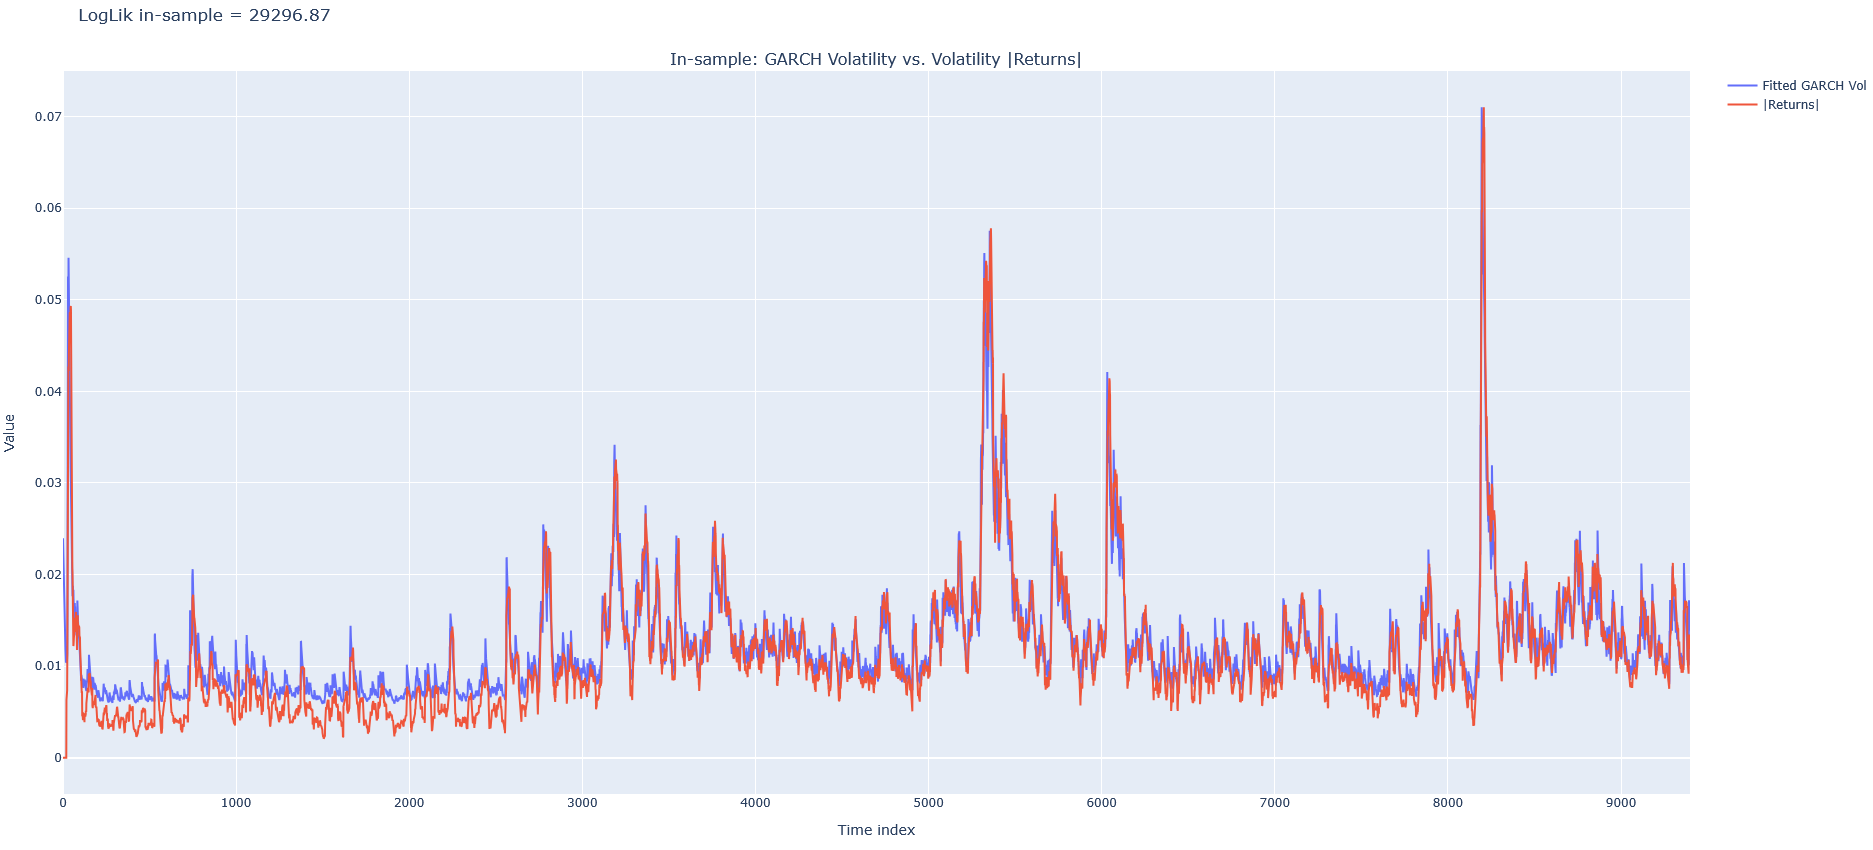
\includegraphics[width=0.8\textwidth]{img/garch_vol}
    \caption{Fitted volatility in sample and volatility of Russell  2000 returns, with garch(1,1).}
    \label{fig:garch_fitted_vol}
\end{figure}

\FloatBarrier

RMSE between GARCH volatility and realized volatility = 0.0023021519154493224 \\

Correlation coefficient GARCH = 0.9615264660690124 \\
